\documentclass[11pt,fleqn,twoside]{article}
\usepackage{makeidx}
\makeindex
\usepackage{palatino} %or {times} etc
\usepackage{plain} %bibliography style 
\usepackage{amsmath} %math fonts - just in case
\usepackage{amsfonts} %math fonts
\usepackage{amssymb} %math fonts
\usepackage{lastpage} %for footer page numbers
\usepackage{fancyhdr} %header and footer package
\usepackage{report} 
\usepackage{url}
\usepackage{cite}
\usepackage[acronym,toc]{glossaries}
\usepackage{float}
\usepackage{graphicx}
\usepackage{pdfpages}

\begin{document}

\name{Luke Ward}
\userid{luw9}
\projecttitle{MapWars: A Location-Aware \\ Multiplayer Strategy Game}
\projecttitlememoir{Location-aware multiplayer strategy game} %same as the project title or abridged version for page header
\reporttitle{Progress Report}
\version{1.1}
\docstatus{Release}
\degreeschemecode{G401}
\degreeschemename{Computer Science}
\modulecode{CS39440}
\supervisor{Reyer Zwiggelaar} % e.g. Neil Taylor
\supervisorid{rzz}

%optional - comment out next line to use current date for the document
% \documentdate{October 20, 2012}

\makeglossaries
\newglossaryentry{restful}{name={REpresentational State Transfer (REST)}, description={is a stateless transfer protocol that has been predominantly used for web applications}}
\newglossaryentry{pull}{name={PULL}, description={is a communication method in which a client requests information from the server every time it needs updates. This means that clients can make numerous requests and get no updates as there is nothing to update. Even when there are available updates it can take time for the client to be updated depending on the interval between requests}}
\newglossaryentry{push}{name={PUSH}, description={is a communication method when a connection is kept open between the client and server, with the server pushing information to the client when updates are available. ThiSpirals means that the server will only send data when there is something to update and with  little latency}}
\newglossaryentry{polling}{name={long polling}, description={This is similar to a standard PULL request but if the server does not have any data to respond with it will keep the connection open until it becomes available}}
\newacronym{rts}{RTS}{real-time strategy}
\newacronym{mmo}{MMO}{massively multiplayer online}
\newacronym{mmorpg}{MMORPG}{massively multiplayer online role playing game}
\newacronym{sdk}{SDK}{software development kit}
\newacronym{rest}{REST}{REpresentational State Transfer}
\newacronym{gcm}{GCM}{Google Cloud Messaging for Android}
\newacronym{vps}{VPS}{virtual private server}

\mmp

%==============================================================================
\section{Project Summary}
%==============================================================================
\subsection{Overview}
MapWars will be a \gls{rts} games based around the users real location and surroundings. With all game play taking place on a map of the real world. It will be built to run on the Android mobile platform with a scalable server to handle control, communication and persistence of the game. This will consist of a single persistent game where every members units are on the same map as everyone else's, including those that are not currently online.

Players will be in command of both units and structures. There will be a variety of unit and structure types, each with their own subtypes with unique advantages and features. These units will only be controllable within a certain range of the players actual location. This range will vary on upgrades and unit type. Units will take the form of infantry, ground and air with each of these having a different subtypes. Each unit will have unique statistics controlling their speed, effectiveness, defences and health. These can increase during action, effectively levelling up with experience. Units will attack enemies units and structures when they come into range, this avoids any complicated controls that can be hard to handle on a small device. Players can select units and move them between locations by simply tapping on the target location. The server will then handle path finding to the given location. An idea that would be nice to tie into this is the use of a navigation API that can provide routes that will follow real world roads and paths. Air units will not be required to follow these routes.

As well as different movable units there will also be a variety of different structures, for example:\begin{itemize}
\item Mines - collect and process resources
\item Power stations - structures will stop functioning if power demands are not met
\item Barracks - used to create ground units
\item Factory - creating ground vehicles
\item Airport - making and replenish air units
\item Command post - extend broadcast coverage
\item Defence - selection of different defensive structures
\end{itemize}
Most structures will have upgrade capabilities that will increase their speed of production, range, effectiveness. 

Resources will be placed all over the world, these resources can be gathered by specialised unit types. Resources will then be used when building structures and units. As resources are collected they will deplete but will regrow in around 24 - 48 hours. I would like to be able to map the location of resources to places in the real world, for example over woodlands. This would allow users to know roughly where resources can be found before they have visited that area. Allowing for planning tactics and even looking at other maps to try and estimate where these maybe placed.

\subsection{Similar Systems}
\subsubsection{Real-Time Strategy Games}
There are a number of \gls{rts} games for the desktop and console gaming market. One of the earliest in this genre Cytron Masters, which was released in 1982, and had many of the features of a modern day game. Two players would be placed on a grid which contained a number of generators, These generators would created resources allowing the players to create different types of units to destroy the enemy. Since then games have built on these fundamental ideas improving graphics, adding features and increasing the number of options presented to the player. The more options available to the player means the more choices they can make and increases the importance of a strong strategy to outwit and overpower the opponent. Advancements in graphical performance of personal computers has seen games evolve from top-down grid based games to isometric and on to fully 3D game-play.

Command \& Conquer became the first multiplayer \gls{rts} when it was released in 1995 for MS-DOS offering network based games with four players. It was later re-released with added internet based multiplayer. As the spread of internet access and its  bandwidth increased so did the popularity of these muliplayer online \gls{rts} games. Even with widespread multiplayer games it is still rare to find \gls{rts} games with more than a handful of player at anyone time. Also the majority of these still take place over a relatively short period of time, with only a handful being persistent even when the user is not online. One game that combines a persistent universe and \gls{mmo} game play is EVE Online. EVE is a \gls{mmorpg} where players control spaceships in a single universe populated with 300,000 other players. The universe consists of over 7,500 solar systems different virtual solar systems. Although the game consists an amount of combat its main focus is on resources and trading via a free and active economy. So even in the wide variety of desktop based \gls{rts} games there is little in the way of a \gls{mmo} game that is both persistent and has a strong emphasis on strategy or tactical based game play.

As for Android offerings in the \gls{rts} market they are few in number and appear to be lacking in certain features. The majority of these are single player medieval games, Medieval Empires\footnote{Medieval Empires - https://play.google.com/store/apps/details?id=com.centralbytes.medievalempires} is a good example of current offerings. This is a solid game but does lack features such as resource gathering. The closest current release to MapWars is Rusted Warfare\footnote{Rusted Warfare - https://play.google.com/store/apps/details?id=com.corrodinggames.rts}, in terms of game play and control it is fairly similar to my expectations for MapWars. Again it does not have the gather aspect but it does have a variety of unit types, limited multiplayer (2-8 players), straight forward unit interactions and intelligent combat. 

\subsubsection{Location-Aware Games}
On the other side there are a number of location based games that take advantage of technology but are played in a totally different way to MapWars. A very interesting one is Can You See Me Now?\footnote{Can You See Me Now? - http://www.blasttheory.co.uk/bt/work\_cysmn.html}. Can You See Me Now? mixes real life location based runners with online players. Each game takes place at a specified time and location. Within this location there will be a number of runners, each equipped with a radio and GPS receiver. Players can login via the internet and will be placed at a location in that city. Players can control their player in virtual reality which the runner can see and will try and track them down with the real world location. When a runner becomes within range of a virtual players location that player has been captured and their game is over. This mix of real world locations, real people and virtual characters is an interesting and exciting one. It shows that the real world and technology can combine and add a new variable to existing concepts.

There are also a lot of location based applications on the Android market but only a few location-aware games. These real world offerings tend to consist of capturing the flag style game play or capturing locations by spending the most time there, for example GeoEmpires\footnote{GeoEmpires - http://geoempires.com/}. With each of these captured locations adding to the users score. There appears to be no player vs player location-aware applications.

\subsection{Objectives}
MapWars is going to attempt to combine the the tactical aspects of these systems with a mobile experience tailored to the users surroundings. Adding in multiplayer gameplay will allow each user to interact, attack and defend against enemies as well as affect the landscape they are playing in. Taking as much of the the tactical aspects of other systems with a higher emphasise on resource gathering and long term tactical game play. Try to remove some of the fast paced ”rushing” game play that can be adopted in some \gls{rts} games. Rushing is a tactic in which a team will attack an opponent as quickly as possible as to surprise and overwhelm them. Hoping that the opponent will not have create adequate defences to counter the attack. One of MapWars main focuses in regard to strategy and game play is to have on continuous game, with many opponents. This will encourage players to concentrate on gathering resources and fortifying their base before they can have the fire-power to take on an enemies forces. As resource gathering is a major aspect of the game play, time permitting, I intend to position these resources based on real world locations. For example allowing users to gather wood or other building materials from woodland and forests that exist in the real world. Resource will deplete as users remove them but they will have a fairly short time scale in which they replenish.


%==============================================================================
\section{Current Progress}
%==============================================================================
\subsection{Client}
Installing and configuring the Android \gls{sdk} to work with Eclipse was as straight forward as it could possibly be, with lots of online guides and resources from Google. After getting the \gls{sdk} setup I started to look at building a basic application to get used to the structure and work flow. Due to my background knowledge of Java and after looking at a couple of tutorials I had a basic "Hello World" style application running. I spent some time getting to grips with creating layouts and controlling the different types of elements and how they can be styled.

One of the first things that I looked into implementing was a mapping solution in a basic Android application. These maps will also needed to be able to handle overlays that could be placed on top of a working interactive map. Each overlay would need to contain multiple items or different types that could both appear differently and be moved individually. Due to Android being developed by Google who also own one of the most widely used online mapping systems it seemed like an obvious choice to first investigate Google Maps. I did some simple spike work into the included maps package that comes with the Android \gls{sdk}. Very quickly I had an application with a working map and a simple overlay. I did not investigate to deep into creating more complex overlays at this point. After verifying that this system met the requirements I had set out I wanted to take a closer look at the terms of use and licensing agreement. The Google Maps API licensing page \cite{google_map_license} states that "Your service must be freely and publicly accessible to end users." This could be a problem for any future development that would result in a paid for application. Therefore I intend to stay away from licensed solutions as much as possible.

So I started to look at alternatives that would be as easy to implement but not have the same limitations on usage. OpenStreetMap is a crowdsourced project to create a free map of the world to rival closed paid for alternatives. Data is first collected via a GPS receiver and uploaded to the site, this is then edited to add more information about the uploaded data. Maps are freely editable by any member of the site so they can update, alter and correct their local area allowing it to quickly respond to changes that may take some time to be reproduced by other organizations. It also has received a lot of data through donations from governments and companies interested in helping the open-source mapping community. OpenStreetMap seemed like a good choice due to its open nature and constant refining, but there are no official Android packages and only a handful of third party offerings. For example osmdroid\footnote{Available here http://code.google.com/p/osmdroid/} which is a near complete replacement of the MapView class I had previously been using in the Google offering. This seemed like a good candidate but I continued to look at OpenStreetMap to see if there was anything else that had more support. AOL's MapQuest in July 2010 introduced OpenStreetMap's data into an open-source offering of their service. MapQuest offerings a complete MapView alternative in the form of its Android Maps Api\cite{mapquest}. This API can serve either licensed data or OpenStreetMap data. When using licensed data you can not include it with a non-publicly available application that is not available without charge, just like with the Google Maps API), but you can if you are using OpenStreetMap data.

A nice feature with OpenStreetMap is the ability to customize map tiles using Mapnik. Mapnik allows you to take the underlying data and style it how you wish, creating anything from simple line drawings to shaded relief maps. This will be infeasible with the number of users this application could expect to support as hosting a tile server is expensive and resource intensive. An alternative to this is to use the data to produce simple paths that can be stored on the server and sent to the client. These would highlight areas such as resources that can then be drawn on a map overlay.

Figure \ref{class} shows the current work that I have undertaken for the Android client. It gathers the users location and creates a unit of this location. This unit is then added to the UnitOverlREpresentational State Transferay which is added to the map. The LocationTracker tracks the users location via data received from both the network and GPS. Each time a new location is received it is compared with the last known position. Depending on if it is deemed to be more accurate than the previVPSous location the user unit location might be updated. If the unit is moved the overlay is invalidated to force a call to the draw method. The draw method iterates through its list of units, getting their location and path which is used to draw the unit. Each unit has a different path, depending on its type, which depicts what should be draw on the canvas. Currently these paths are simple 3 or 4 sided shapes but they could easily be swapped out for more complex shapes or even SVG files.

\begin{figure}[H]
\centering
% \input{class.tex}
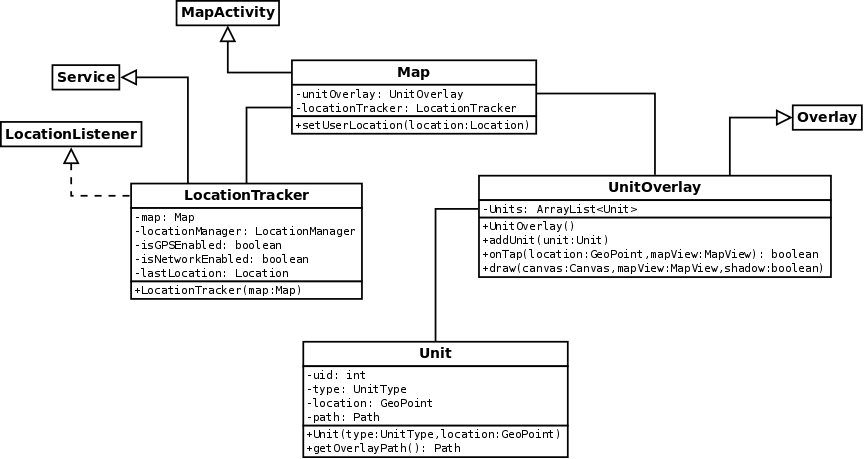
\includegraphics[width=\linewidth]{class}
\caption{Class diagram of currently achieved work}
\label{class}
\end{figure}

\subsection{Server}
Regarding the server portion of the system, I have just started looking into the different technologies and options available to me. I have yet to decide on a language or communication method.

I started of by looking at the advantages and disadvantages of \gls{push} and \gls{pull} communications. Due to the nature of the application I am trying to create the default choice would be to use \gls{push} technology. This would mean that the updates from the server propagate to all the relevant clients as soon as they are created. As well as this  Android does support \gls{push} but only via its own \gls{gcm}, which I need to do further research into. There are a number of ways to achieve similar effects such as \gls{polling} but \gls{gcm} handles a lot of the transmission for you. It is also imposes no quotas and can allow an application to receive messages even when it is not active.

\gls{pull} has the advantage of being easy to implement due to being sent via a standard request. Although the apparent disadvantages of high update latency and increased battery and data usage. I have found an interesting paper about using RESTful architecture for multi-user virtual environments \cite{6329833}. In this study they examined if a \gls{rest} architecture could be used to handle the number of interactions a \gls{mmo} is expected to. Current desktop \gls{mmo} games tend to use tightly coupled interactions between client and server that resulted in limited scalability. They conclude that it is feasible to support the kind of user and interaction loads found in popular \gls{mmo}s using \gls{rest} if caching and other techniques were utilized. \gls{rest} lends itself to scalable applications due to its stateless communication, meaning that it will need to re-authenticate for each request. This re-authentication means that the request can be passed and handled by any server in the network, irrespective of any previous interactions with the client. Creating a scalable server architecture is one of my main goals for the server, using \gls{pull} would make this easier. Each request would be received by a transparent proxy that will forward the message on to one of the servers residing behind it. The server will then process this request, responding data will then relayed back through the proxy to the client. Having each request hit the proxy before being allocated to a server will help load balance the servers, distributing activity equally between servers. Allowing the proxy to avoid overloaded machines until they finish their current requests. When using \gls{push} this balancing becomes more complicated as the proxy will direct each new client to the least loaded server. As users connect and part one server may become overloaded as its connected clients continue to interact heavily while other servers sit idling. This can be combated by closing connections and having them re-established with a different server when one comes under heavy load. Again I am not entirely sure how this will relate to \gls{gcm} as this handles its own connections with the client and any server can push messages onto \gls{gcm}.

I still need to do spike work into implementing both methods before I can come to solid conclusion. I intend to create a basic client and server for both methods, with the client sending variable amounts of test data. This spike work will need to look into the following:
\begin{itemize}
\item Complexity of implementation
\item Battery usage
\item Data usage
\item Latency
\item Server load per client
\item Scaling options
\end{itemize}
I am interested in looking at using \gls{push} over \gls{pull} despite of the possible draw back of power usage and possible latency. The latency issue can be reduced by implementing parts of the server logic into the client. Thus the client can predict what actions have taken place in regards to unit placement, resource gathering etc between updates from the server. The server updates will then replace the predicted data hopefully with limited effect. Avoiding the \gls{gcm} would allow greater control over data transmission and proxy/distribution considerations. As well as this it would be nice to expand on the work described in the RESTful feasibility study \cite{6329833}. Taking the conclusions that they reached and applying them to a real world application to see if it really does scale as well as they predicted. Testing it with multiple proxies and servers and seeing if the same results are seen or if there is a consideration that they missed. On top of this the paper was aimed at the desktop broadband MMO with fast paced interactions, where as MapWars intends to be used slightly differently. With less interactions over a much longer period of time via a greatly reduced connection.

As well as creating a responsive and scalable server it must also be secure and fair. Security in online games can play a big part on how well playable the end game is. A system that can give some users advantages over others is highly undesirable. These advantages can either be malicious or coincidental, some users will find flaws and purposefully exploit them whereas others may have advantage through no action of their own. There are a number of resources I have found that both detail current online game solutions\cite{sec2, sec3} as well as those tailored towards mobile communications\cite{sec1}.

\subsection{Development Environment}
The client portion of this application will be developed in the Eclipse IDE\footnote{Eclipse homepage - http://www.eclipse.org/} utilizing the official Android Development Tools (ADT) plugin\footnote{ADT plugin - http://developer.android.com/tools/sdk/eclipse-adt.html}. As the only supported language for the Android platform it will be written in Java along with the Android \gls{sdk}. The language choice for the server is yet to be decided. Tt will need to have minimal performance overheads so C++ would be an ideal choice, but other options such as Python will need to be considered. Irrespective of language choice I will imagine that I will be using Sublime Text 2\footnote{Sublime homepage - http://www.sublimetext.com/} as my preferred editor. All development will be done on a Debian based linux machine, using a number of Android devices and virtual machines to test compatibility. Current device list is a Motorola Atrix (v2.3.4), Motorola Xoom 2 Media Edition (v4.0.4) and a Sony Ericsson ST25i (v2.3.7). The server and proxy will be running on a number of Debian based linux machines, most likely \glspl{vps}. I will be using a private Git repository hosted by BitBucket for version control and issue/bug tracking.

%==============================================================================
\section{Planning}
%==============================================================================
My development method will consist of taking the project and breaking it into smaller segments that can be tackled individually. Each segment will contain a planning, development and analysis stage. The development will take place iteratively building on prototypes to produce the final component. This will avoid making throwaway prototypes and cut down on development time. These segments will build upon the ones before, building up a complete working application. This combines different aspects from both the Spiral and Rapid application development (R.A.D) methodologies.

A weekly plan has been set out that is currently up until mid-January 2013. It covers the major aspects and milestones of the project as well due dates for each hand in. At the time of writing the first two sections, mapping solutions and location services have both been completed comfortably within time. The next stage is to research, prototype different client-server communication methods. Writing up my findings and implementing the basis of my chosen method. After getting the basic client-server interactions working it will be a case of adding features to each and adding the required supporting system to the other. Adding features until a basic working prototype is ready for testing which I plan to be at the end of November during the last week of term. This basic prototype aims to locate each user and display their location on every users device. It will be an important test on such things as responsiveness, battery usage and server stability and load. Testing will take the form of distributing my test application to a number of testers who will spread out and walk around the local area. Detailed logs will be take on each device storing different hardware events, such as GPS updates and battery statuses, as well as all sent and received data from the server. Also the server and proxy will log all the connections received and responded to as well as their loads at various intervals.

\subsection{Demonstrations}
The first mid-project demonstration will showcase the application in its current state using data and recordings taken from the user testing that took place earlier. This prototype should be handling multiple users and plotting their current locations, this might include a basic unit prototype. New features and improvements can be demonstrated on a live system using server generated test players, units and events. Hopefully for the final demonstration I will have willing test players around the local area actively playing the game during the demonstration. Both a client view and server view can then be presented to show what is happening, with the client being able to join the action within any players with range. Again server generated players and events may also be used to simulate more concurrent players. There will be a fully fledged unit and combat system with multiple unit types. As well as structures, resource gathering and path finding.



\glsaddall
\printglossaries

\addcontentsline{toc}{section}{Annotated Bibliography}
% example of including
\nocite{*}

\bibliographystyle{IEEEannot}
\renewcommand{\refname}{Annotated Bibliography}  % if you put text into the final {} on this line, you will get an extra title, e.g. References. This isn't necessary for the outline project specification. 
\bibliography{report} % References file

\newpage
\thispagestyle{empty}
\appendix
\section{Gantt Chart}
\center
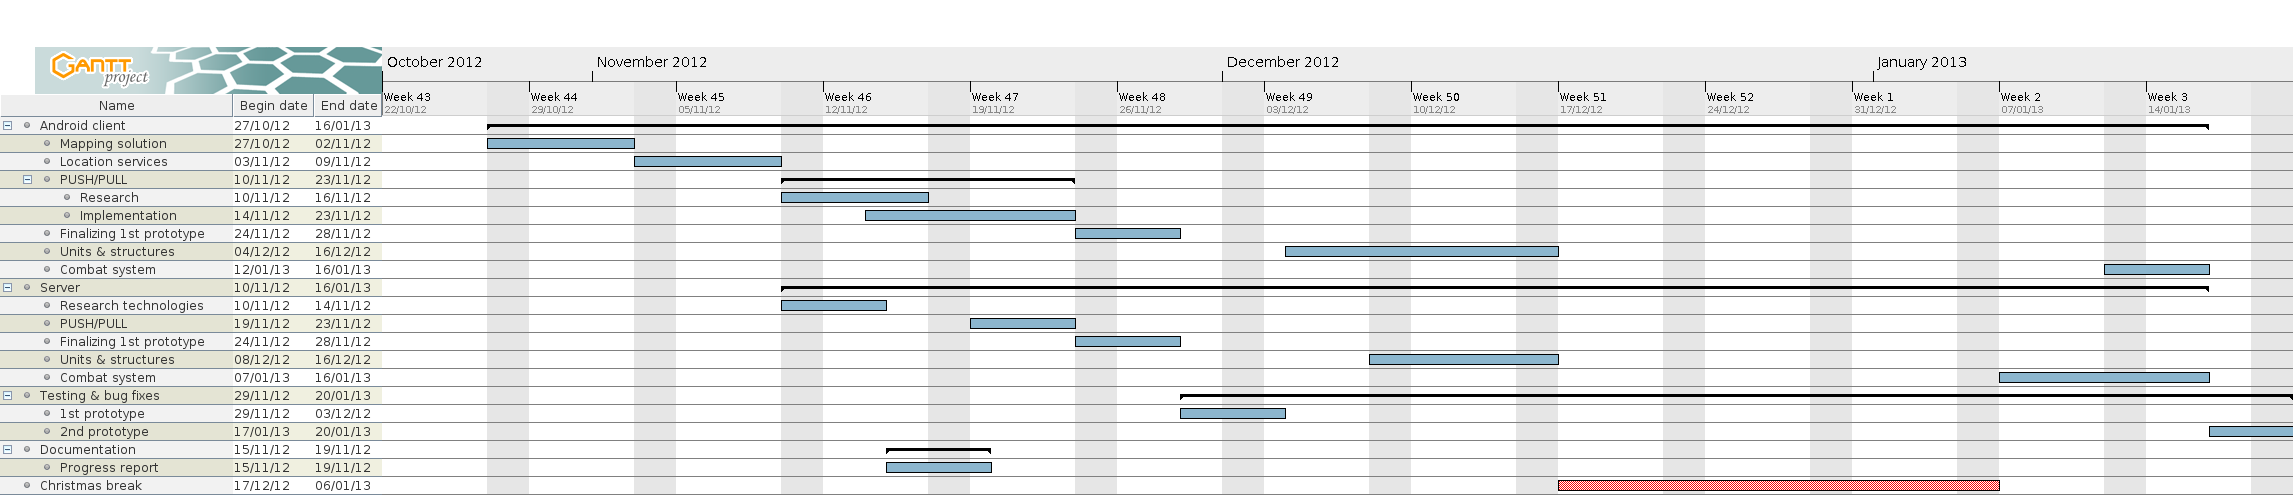
\includegraphics[angle=-90,totalheight=\textheight]{weekly-plan.png}
% \includepdf[landscape=true,pages={3}]{../weekly-plan.pdf}



\end{document}
